\documentclass[10pt,a4paper]{report}
\usepackage[utf8]{inputenc}
\usepackage[russian]{babel}
\usepackage{amsmath}
\usepackage{amsfonts}
\usepackage{amssymb}
\usepackage{graphicx}
\renewcommand{\thesection}{\arabic{section}}
\setcounter{totalnumber}{10}
\setcounter{topnumber}{10}
\setcounter{bottomnumber}{10}
\renewcommand{\topfraction}{1}
\renewcommand{\textfraction}{0}
\author{Евсеев Дмитрий}
\title{Лабораторная работа №5.\\
	SSL/TSL}

\begin{document}
\maketitle
\tableofcontents
\pagebreak

\section{Цель работы}

Сервис тестирования корректности настройки SSL на сервере Qualys SSL Labs – SSL Server Test

\section{Ход работы}

\subsection{Лучшие практики по развертыванию SSL}

\begin{itemize}
	\item Использовать 2048-битные закрытые ключи.
	Использовать 2048-битный RSA или 256-битные ECDSA закрытые ключи для всех серверов. Ключи такой крепости безопасны и будут оставаться безопасными в течение значительного периода времени.
	\item Защитить закрытый ключ. Относитесь к закрытым ключам как к важным активам, предоставляя доступ к как можно меньшей группе сотрудников.
	\item Обеспечить охват всех используемых доменных имен. Убедитесь, что ваши сертификаты охватывают все доменные имена, которые вы хотите использовать на сайте.
	\item Приобретать сертификаты у надежного удостоверяющего центра (CA).
	\item Использовать надежные алгоритмы подписи сертификата. Безопасность сертификата зависит от длины закрытого ключа и прочности используемой функции хеширования. Сегодня большинство сертификатов используют алгоритм SHA1, который считается слабым. 
	\item Использовать безопасные протоколы. (TLS v1.0/v1.1/v1.2)
	\item Использовать безопасные алгоритмы шифрования. В данном случае подойдут симметричные алгоритмы с ключами более 128 бит.
	\item Контролировать выбор алгоритма шифрования. В SSL версии 3 и более поздних версиях протокола, клиенты отправляют список алгоритмов шифрования, которые они поддерживают, и сервер выбирает один из них для организации безопасного канала связи. Не все сервера могут делать это хорошо, так как некоторые выбирают первый поддерживаемый алгоритм из списка.
	\item Использование Forward Secrecy. Forward Secrecy — это особенность протокола, который обеспечивает безопасный обмен данными, он не зависит от закрытого ключа сервера. С алгоритмами шифрования, которые не поддерживают Forward Secrecy, возможно расшифровать ранее зашифрованные разговоры с помощью закрытого ключа сервера.
	\item Отключить проверку защищенности по инициативе клиента.
\end{itemize}

\subsection{Основные уязвимости и атаки на SSL}

\paragraph {POODLE\\}
Атака POODLE(Padding Oracle On Downgraded Legacy Encryption) работает по следующему сценарию: Взломщик отправляет свои данные на вервер по протоколу SSL3 от имени взламываемой структуры, что позволяет ему постепенно расшифровывать данные из запросов. Это возможно, так как в SSL3 нету привязки к MAC адресу.

\paragraph {Heartbleed\\}
Ошибка (переполнение буфера) в криптографическом программном обеспечении OpenSSL, позволяющая несанкционированно читать память на сервере или на клиенте, в том числе для извлечения закрытого ключа сервера. Информация об уязвимости была опубликована в апреле 2014 года, ошибка существовала с конца 2011 года.

\subsection{Домен из списка Recent Best}

Cо стартовой страницы SSL Server Test выбран один домен из списка Recent Best (рисунок \ref{Img:1}).

\paragraph {Recent Best\\}

\begin{figure}[h!]	
	\center{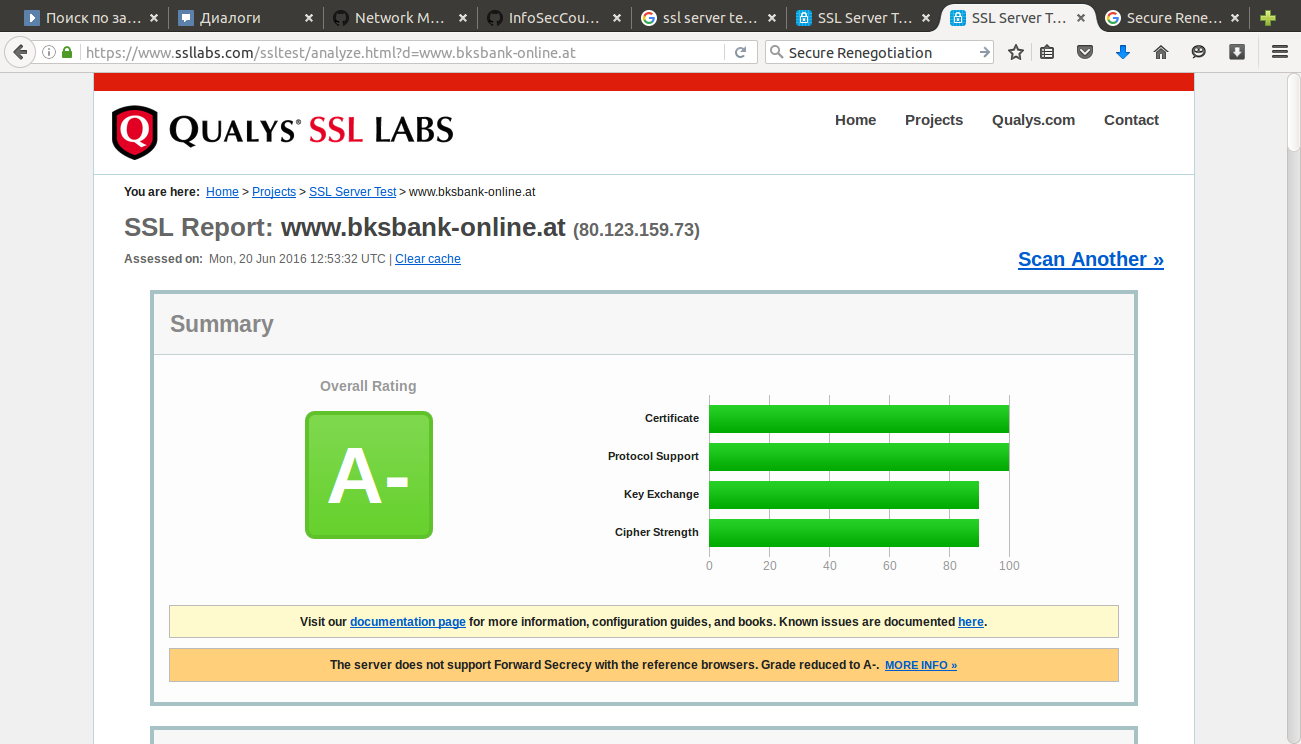
\includegraphics[width=0.8\linewidth]{Img/1}}
	\caption{Summary для recent best.}
	\label{Img:1}
\end{figure}

\begin{itemize}
	\item Поддержка TLS 1.2
	\item Не поддерживает небезопасный SSL v3
	\item Поддержка Secure Renegotiation
\end{itemize}

\subsection{Домен из списка Recent Worst}

Summary для домена из Recent worst (рисунок \ref{Img:2})

\paragraph {Recent Worst\\}

\begin{figure}[h!]	
	\center{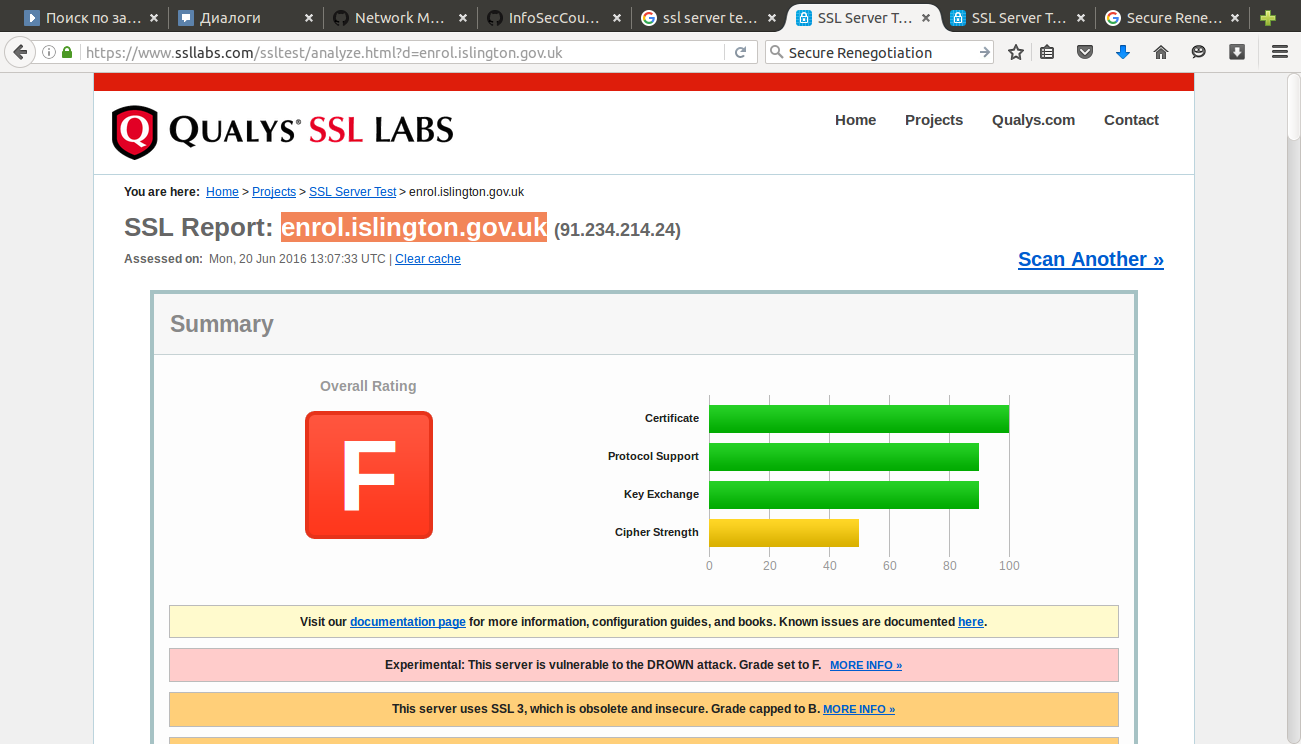
\includegraphics[width=0.8\linewidth]{Img/2}}
	\caption{Summary для recent worst.}
	\label{Img:2}
\end{figure}

\begin{itemize}
	\item Поддерживает небезопасный SSL v3
	\item Подвержен DROWN атакам
	\item Использует небезопасный RC4
	\item Не поддерживает Forward secrecy 
\end{itemize}

\subsection{Выбор интернет-домена, защищенного SSL-шифрованием.}
Для анализа защищенности SSL шифрованием был выбран домен youtube.com (рисунок \ref{Img:3}).

\begin{figure}[h!]	
	\center{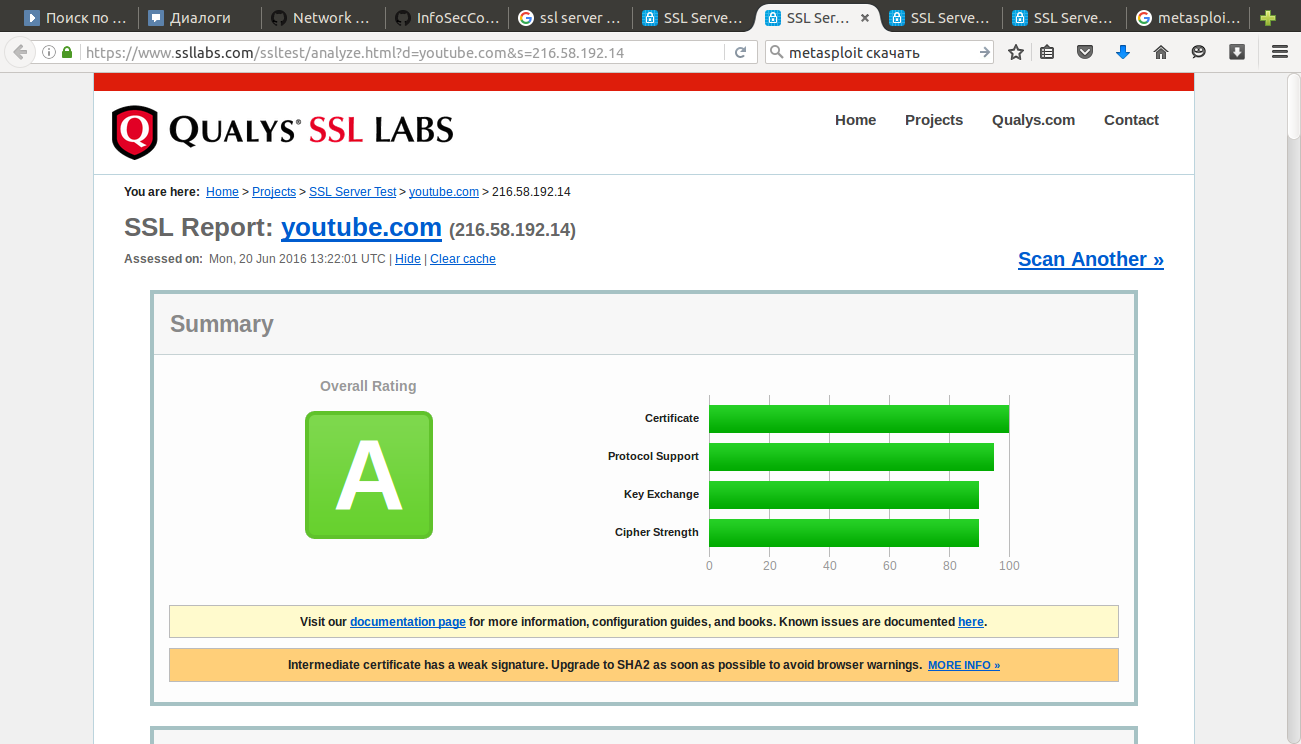
\includegraphics[width=0.8\linewidth]{Img/3}}
	\caption{Summary для youtube.com.}
	\label{Img:3}
\end{figure}
\pagebreak

\paragraph{Configuration\\}

\begin{figure}[h!]	
	\center{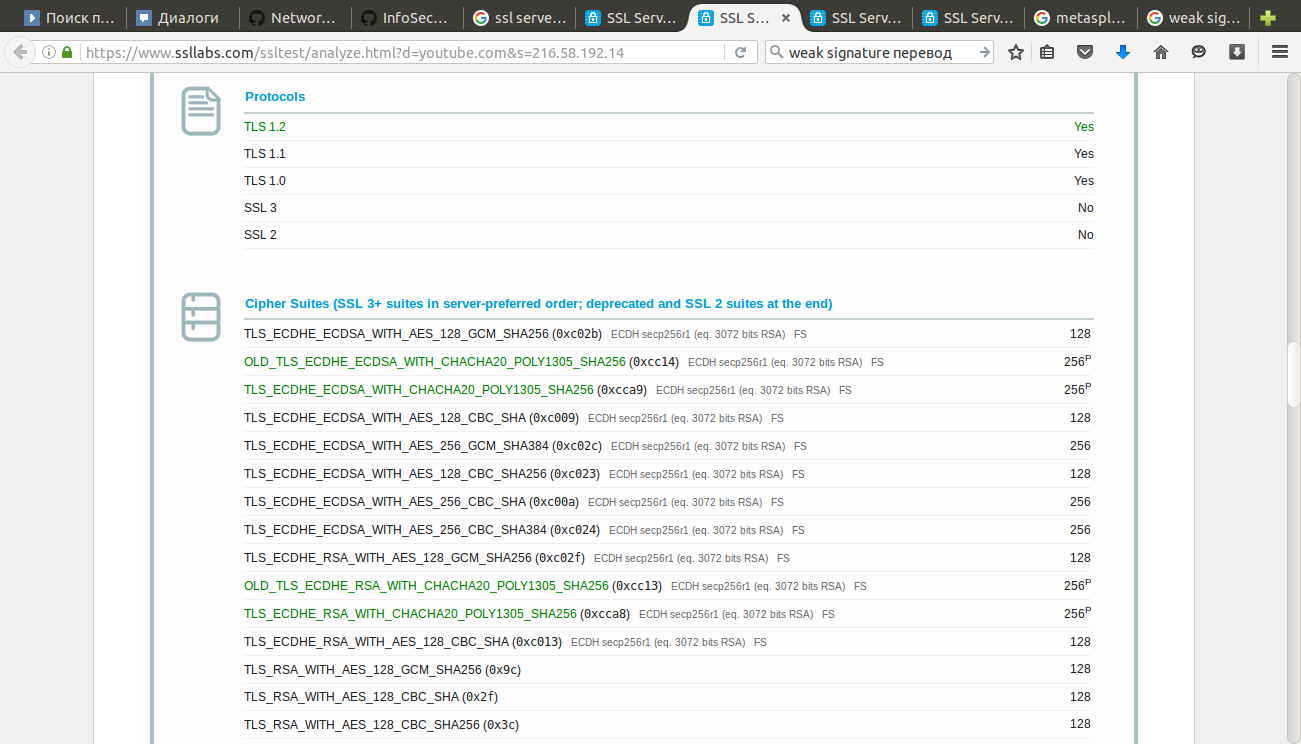
\includegraphics[width=0.8\linewidth]{Img/4}}
	\caption{Configuration для youtube.com.}
	\label{Img:4}
\end{figure}

\begin{itemize}
	\item{ECDH - Elliptic curve Diffie–Hellman - Протокол Дииффи-Хееллмана на эллиптических кривых}
	\item{RSA - Rivest, Shamir, Adleman - криптографический алгоритм}
	\item{RC4 - Rivest Cipher 4 -  потоковый шифр 4-й версии}
	\item{SHA/SHA256/384 - Secure Hash Algorithm - Алгоритм хэширования. Цифра - длина ключа}
	\item{AES - Advanced Encryption Standard - симметричный алгоритм блочного шифрования}
	\item{GCM и CBC это два режима блочного шифрования}
	\item{TLS - Transport Layer Security - криптографический протокол}
	\item{3DES - Digital Encryption Standard - алгоритм блочного шифрования}
	\item{EDE - Encrypt, Decrypt, Encrypt - режим работы алгоритма 3DES}
\end{itemize}

\paragraph{Protocol details\\}

\begin{figure}[h!]	
	\center{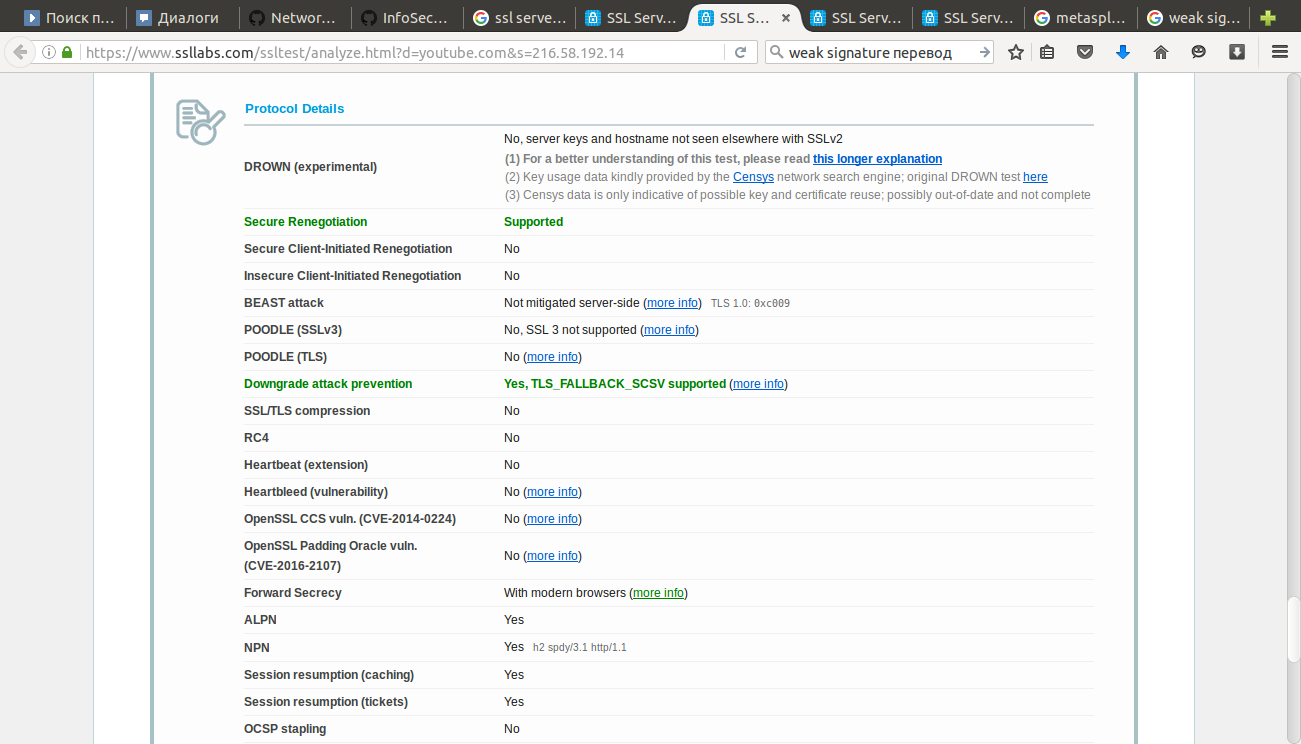
\includegraphics[width=0.8\linewidth]{Img/5}}
	\caption{Protocol details для youtube.com.}
	\label{Img:5}
\end{figure}

\begin{itemize}
	\item{Secure Renegotiation - Возобновление подлючения TLS}
	\item{Secure Client-Initiated Renegotiation, Insecure Client-Initiated Renegotiation - подверженность процесса проверки сертификата атаке.}
	\item{BEAST attack, POODLE (SSLv3), POODLE (TLS) - проверка уязвимости к данным атакам.}
	\item{Downgrade attack prevention - атака, при которой клиента принудительно заставляют использовать предыдущие (менее надежные) версии протоколов}
	\item{SSL/TLS compression - сжатие SSL/TLS не используется}
	\item{RC4 - Не спользуется слабый шифр RC4}
	\item{Heartbeat (extension), Heartbleed (vulnerability), OpenSSL CCS vuln. (CVE-2014-0224) - уязвимости OpenSSL Heartbleed и тд.}
	\item{Forward Secrecy - совместимость Forward Secrecy с новыми браузерами.}
	\item{Strict Transport Security (HSTS) - форсированное переключение на HTTPS}
	\item{SSL 2 handshake compatibility - Совместимость с SSL 2 handshake}
\end{itemize}

\subsection{Вывод о реализации SSL на youtube.com}

Общую защищенность сервера можно оценить как отличную. Все характеристики удовлетворяют лучшим практикам развертывания SSL.

\section{Выводы}
В результате выполнения работы были изучены лучшие практики по развертыванию SSL серверов, а так же средство для проверки SSL серверов Qualys SSL Server Test, которое позволяет подробно изучить любой домен. Полученные данные помогут получить действительную картину защищенности сервера и понять какие действия необходимо препринять для улучшения стабильности и безопасности сервера.

\end{document}